\documentclass[report]{../../custom}
\begin{document}
\maketitle

\noindent \textbf{摘要:} 对SPHINCS+签名算法并行化实现策略的深入研究。借助文献 \cite{Wang2025} 的理论探讨与实验数据,我们对HT树、FORS树及WOTS+算法的并行化方案进行了详细剖析,并评估了最大与最小并行化策略在实际运用中的性能表现与局限性。此外,明确了在GPU平台上复现相关实验的初步计划,并针对如何优化系统整体性能提出了未来的研究方向。

\vskip 0.5cm

\noindent \textbf{下周计划:} 1) 复现 \cite{Wang2025} 实验;2) 调整HASH运算分组数,提升并行效率;3) 将签名算法应用于实际场景中。

\section{论文阅读}

本周我们深入研读了 \cite{Wang2025},该论文系统性地探讨了如何并行化实现SPHINCS+签名算法。文中详细阐述了针对HT树、FORS树及WOTS+算法的并行化策略,并依据各组成部分的执行顺序提出了一种分层并行方案,共划分为四个层次。由于各层之间相对独立,该文提出的组合并行策略可根据具体资源情况灵活调整,从而实现\textcolor{blue}{更高的并行效率(PE)},即 PE=效率/资源。

具体而言,如图 \ref{fig:merkle_tree_paralle} 所示,左侧示例展示了最大并行化情形,即将每次HASH运算视为独立任务,但由此引入了四次同步操作,导致计算负载不均衡并引发等待现象;而右侧示例则采用最小并行化策略,将所有HASH运算合并为两个任务,虽然有效缓解了负载不均问题,但并行度则显著降低。因此,我们计划在这两种策略之间寻求一个\textcolor{blue}{合适的HASH运算分组数},以实现计算负载与并行度之间的最佳折中,并由此提升PE。

\begin{figure}[!ht]
\centering
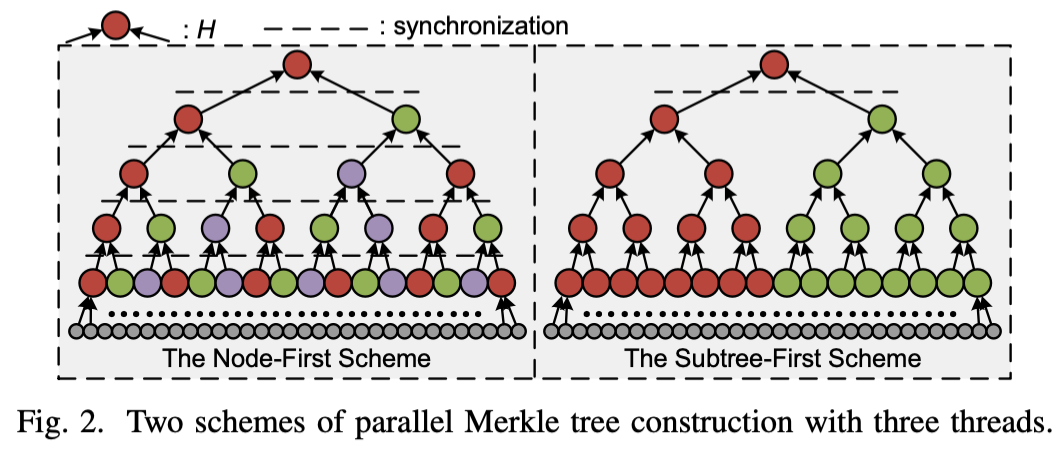
\includegraphics[width=0.6\textwidth]{./fig/merkle_tree_paralle.png}
\caption{Merkle Tree 并行化\cite{Wang2025}}
\label{fig:merkle_tree_paralle}
\end{figure}

在获得 \cite{Wang2025} 源代码的基础上,我们将着手在GPU平台上复现其实验,并在此基础上进行进一步的优化,以提升系统总体性能。同时,考虑将签名算法应用于实际场景中。

\bibliographystyle{alpha}
\bibliography{../../paper}

\end{document}